\documentclass[12pt]{article}

\usepackage[brazilian]{babel}
\usepackage[utf8]{inputenc}
\usepackage[T1]{fontenc}
\usepackage{graphicx}
\everymath{\displaystyle}
\usepackage{amssymb}



\begin{document}
\date{}
\title{1ª PROVA DE CÁLCULO}
\author{Prof. Viviane Ribeiro Tomaz da Silva}
\maketitle

\part{Enunciados}
\begin{enumerate}
	\item (9,0 pontos) Determine:
	\begin{enumerate}
		\item $ \lim\limits_{x \rightarrow 0}(e^x - 1) \sin({ e^\frac{1}{x}}) $
		\item $ \lim\limits_{x \rightarrow \infty} \sqrt{x^2 - 5x} - \sqrt{x^2 - 3} $
		\item as assíntotas verticais de $ f(x) = \frac{3x^2 + 4}{x^2 - 1} $, calculando os limites correspondentes.
	\end{enumerate}
	\item (4,0 pontos) Determine o valor de $c$ que torna contínua a função \\
	$ \left\{\begin{array}{ll} \frac{\sin{(cx)} }{2x}$, se $  x\not=0 \\ 3 $, se $  x = 0 \end{array}\right\} $.
	\item (9,0 pontos) Encontre a derivada de $ f(x) = \frac{e^x x^4}{\cos{x}} + \ln{(8+\tan{x})} $.
	\item (7,0 pontos) Considere a função $ f(x) = \sqrt[7]{x^3 - 12x} $.
	\begin{enumerate}
		\item Determine todos os pontos do gráfico de $f$ nos quais a reta tangente ao gráfico é horizontal.
		\item Em que pontos a função $f$ é derivável?
	\end{enumerate}
	\item (4,0 pontos) Considere a função $ f(x) = x^2 - x -2 $. Mostre que $f(x)$ possui pelo menos duas raízes reais distintas.
\end{enumerate}

\newpage
\part{Resolução}
\begin{enumerate}
	\item (9,0 pontos) Determine:
	\begin{enumerate}
		\item $ \lim\limits_{x \rightarrow 0}(e^x - 1) \sin({ e^\frac{1}{x}}) $ \\
		\\
		Sabemos que a função $\sin({ e^\frac{1}{x}})$ se comportará oscilando no intervalo $[-1,1]$, mesmo que o expoente de $e$ tenda ao infinito quando $x \rightarrow 0$ a função continuará limitada no intervalo.\\ \\
		Analisando agora o trecho $ (e^x - 1) $ temos que $e^x$ é contínuo no seu domínio nos reais, e $e^0 = 1$, com isso podemos inferir que:\\
		\begin{center}
			$ \lim\limits_{x \rightarrow 0}(e^x - 1)(-1) \le
			\lim\limits_{x \rightarrow 0}(e^x - 1) \sin({ e^\frac{1}{x}}) \le
			\lim\limits_{x \rightarrow 0}(e^x - 1)(1) $
			\\
			$ 0 \le \lim\limits_{x \rightarrow 0}(e^x - 1) \sin({ e^\frac{1}{x}}) \le 0 $
			\\
			$ \lim\limits_{x \rightarrow 0}(e^x - 1) \sin({ e^\frac{1}{x}}) = 0 $
		\end{center}
		
		\begin{center}
			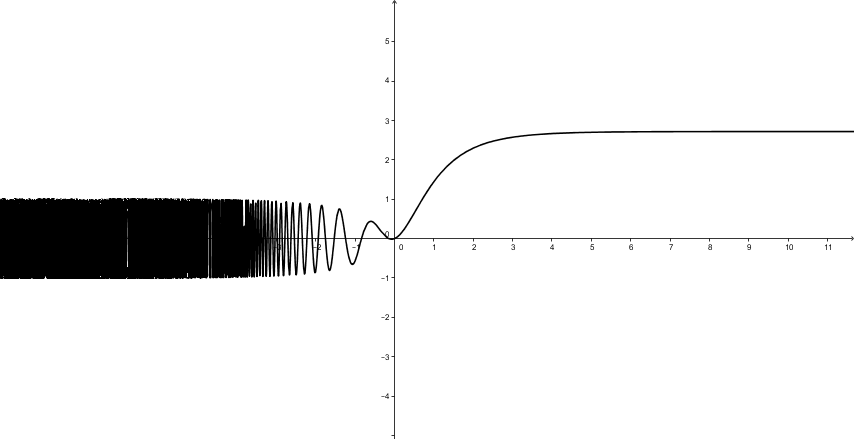
\includegraphics[scale=1.5]{img/1.png}
		\end{center}
		
		
		\item $ \lim\limits_{x \rightarrow \infty} \sqrt{x^2 - 5x} - \sqrt{x^2 - 3} $
		\\
		\\
		Primeiramente, vamos observar se não existem problemas no domínio da função ao tender a infinito, note que:\\
		\begin{center}
			$ x^2 - 5x \ge 0 \rightarrow x \ge 5 $\\
			$ x^2 - 3 \ge 0 \rightarrow x \ge \sqrt{3} $\\
		\end{center}
		Como não infinito está além dessas restrições seguimos tentando desenvolver a expressão multiplicando pelo conjugado:\\
		\begin{center}
			$\lim\limits_{x \rightarrow \infty} \sqrt{x^2 - 5x} - \sqrt{x^2 - 3}=$	
			\\		
			$\lim\limits_{x \rightarrow \infty} \frac{-5x + 3}{ \sqrt{x^2 - 5x} + \sqrt{x^2 - 3}} =$
			\\
			$\lim\limits_{x \rightarrow \infty} \frac{x \left(-5 + \frac{3}{x} \right) }{ x \left(\sqrt{1 - \frac{5}{x^2}}\right) + x \left(\sqrt{1 - \frac{3}{x^2}}\right)} =$
			\\
		\end{center}
		O $x$ em evidência pode ser cortado, os termos múltiplos que possuem $x$ no denominador e uma constante no numerador vão tender a zero, então temos:
		\begin{center}
			$\lim\limits_{x \rightarrow \infty} \frac{\left(-5 + 0 \right) }{ \left(\sqrt{1 - 0}\right) + \left(\sqrt{1 - 0}\right)} =
			\frac{-5}{2}$
			\\
		\end{center}	
		
		\begin{center}
			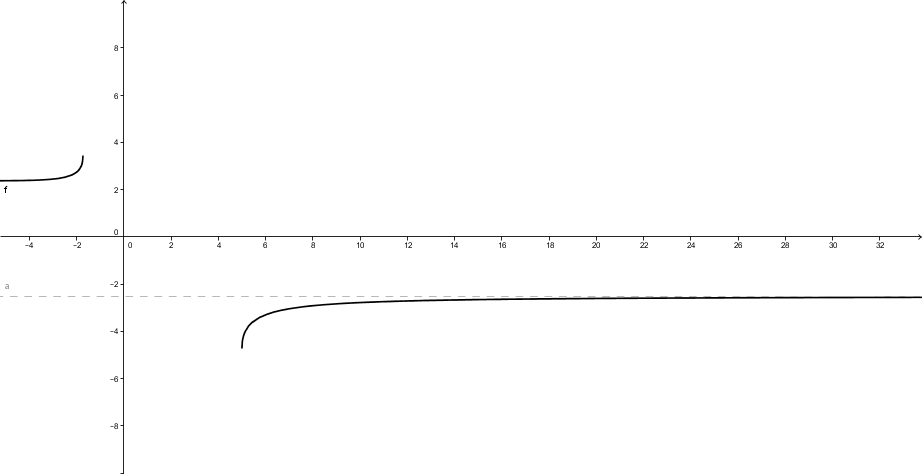
\includegraphics[scale=1.5]{img/2.png}
		\end{center}
		
		
		\item as assíntotas verticais de $ f(x) = \frac{3x^2 + 4}{x^2 - 1} $, calculando os limites correspondentes.\\
		\\
		Assíntotas verticais surgem de divisões por zero em pontos ($a$) indeterminados e possuem equação na forma $x = a$. A função dada é indeterminada quando o denominador é zero, logo:
		\begin{center}
			$x^2 - 1 = 0 \rightarrow x = \pm 1$
			\\
		\end{center}
		Vamos verificar os limites laterais (para entender o sinal basta fazer um estudo do sinal com a função do numerador e do denominador para entender o comportamento da divisão):
		\begin{center}
			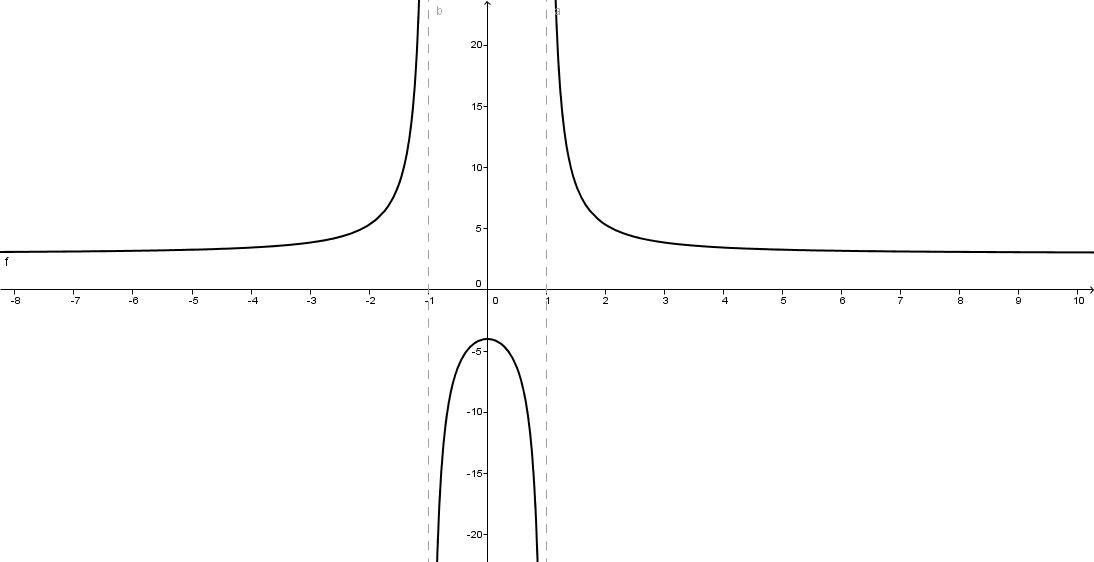
\includegraphics[scale=1.2]{img/3.png}
		\end{center}
		\begin{center}
			$\lim\limits_{x \rightarrow 1^{+}} \frac{3x^2 + 4}{x^2 - 1} = +\infty $
			\\
			$\lim\limits_{x \rightarrow 1^{-}} \frac{3x^2 + 4}{x^2 - 1} = -\infty $
			\\
			$\lim\limits_{x \rightarrow -1^{+}} \frac{3x^2 + 4}{x^2 - 1} = -\infty $
			\\
			$\lim\limits_{x \rightarrow -1^{-}} \frac{3x^2 + 4}{x^2 - 1} = +\infty $
		\end{center}
		
	\end{enumerate}
	\item (4,0 pontos) Determine o valor de $c$ que torna contínua a função \\
	$ \left\{ \begin{array}{ll} \frac{\sin{(cx)}}{2x} $, se $ x \not= 0 \\ 3 $, se $ x = 0 \end{array}\right\} $ .\\
	\\
	\begin{center}
		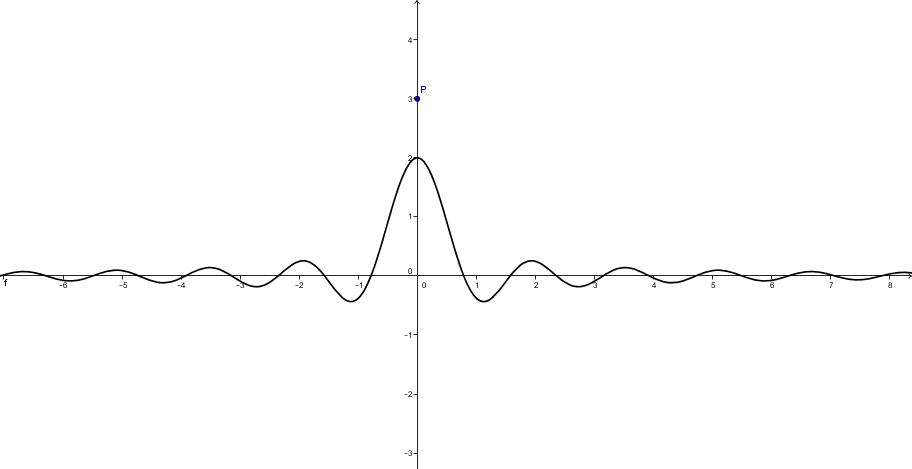
\includegraphics[scale=1.5]{img/4.png}
	\end{center}
	
	O objetivo desse exercício é encontrar o valor de c que faz com que a função dada "passe" pelo ponto fixo $(0,3)$ tornando a função contínua. Logo:
	\begin{center}
		$\lim\limits_{x \rightarrow 0} \frac{\sin{(cx)}}{2x} = 3 $ \\
		$\lim\limits_{x \rightarrow 0} \frac{\sin{(cx)}}{6x} = 1 $ \\
	\end{center}
	\begin{center}
		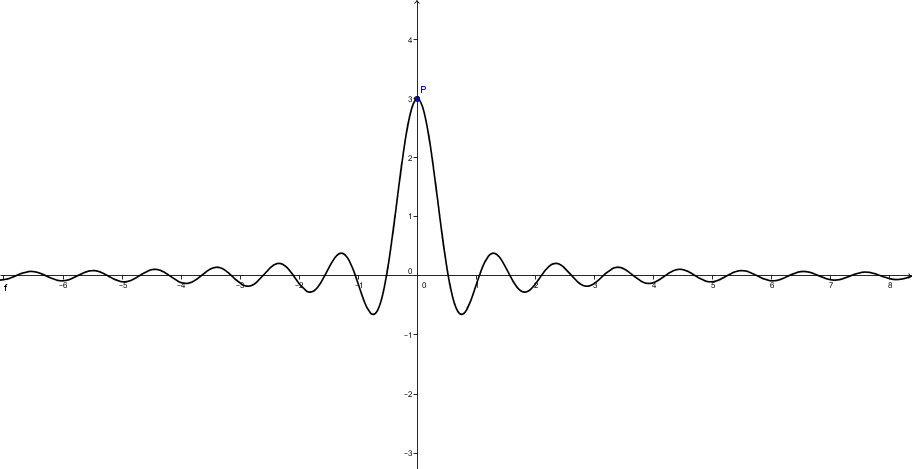
\includegraphics[scale=1.5]{img/4ok.png}
	\end{center}
	Sabemos que:
	\begin{center}
		$\lim\limits_{x \rightarrow 0} \frac{\sin{(x)}}{x} = 1 $
	\end{center}
	Então $c = 6$.\\
	
	
	\item (9,0 pontos) Encontre a derivada de $ f(x) = \frac{e^x x^4}{\cos{x}} + \ln{(8+\tan{x})} $.\\
	\\
	Enumerando as regras utilizadas:
	\begin{center}
		$ \left[\frac{f(x)}{g(x)}\right]' = \frac{f'(x)g(x) - f(x)g'(x)}{g(x)^2} $\\
		$ \left[f(x)g(x)\right]' = f'(x)g(x) + f(x)g'(x) $\\
		$ \left[f(x)+g(x)\right]' = f'(x) + g'(x) $\\
		$ [fog]' = f'(g(x))g'(x) $\\
	\end{center}
	
	\begin{center}
		$ \left[\frac{e^x x^4}{\cos{x}}\right]' = \frac{(e^x x^4 + 4e^x x^3)\cos x + (\sin x)(e^x x^4)}{\cos^{2}x} $\\
		$ \left[ ln{(8+\tan{x})} \right]' = \frac{\sec^{2}x}{8 + \tan x} $\\
	\end{center}
	
	\begin{center}
		$ f'(x) = \frac{(e^x x^4 + 4e^x x^3)\cos x + (\sin x)(e^x x^4)}{\cos^{2}x} + \frac{\sec^{2}x}{8 + \tan x} $\\
	\end{center}
	
	
	
	\item (7,0 pontos) Considere a função $ f(x) = \sqrt[7]{x^3 - 12x} $.
	\begin{enumerate}
		\item Determine todos os pontos do gráfico de $f$ nos quais a reta tangente ao gráfico é horizontal.\\
		\\
		Uma reta é horizontal quando seu coeficiente angular é nulo, como a derivada é o coeficiente angular da reta em um ponto temos que derivar e igualar a zero:
		
		\begin{center}
			$ f(x) = \left[\sqrt[7]{x}\right]' = \frac{1}{7}x^{\frac{-6}{7}} $\\
			$ g(x) = \left[x^3 - 12x\right]' = 3x^2 - 12 $\\
			$ [fog]' = f'(g(x))g'(x) $\\
			$ \left[\sqrt[7]{x^3 - 12x}\right]' = \frac{1}{7}(x^3 - 12x)^{\frac{-6}{7}}(3x^2 - 12)  $\\
		\end{center}
		\begin{center}
			$ \frac{3x^2 - 12}{7(x^3 - 12x)^{\frac{6}{7}}} = 0  $\\
			$ 3x^2 - 12 = 0  $\\
			$ x = \pm 2  $\\
		\end{center}
		
		É importante, também, que o denominador não seja zerado pelos valores obtidos, observe:
		
		\begin{center}
			$ 7((2)^3 - 12(2))^{\frac{6}{7}} \not= 0 $\\
			$ 7((-2)^3 - 12(-2))^{\frac{6}{7}} \not= 0 $\\
		\end{center}
		
		Note que $x^3 - 12x$ pode ser menor que zero, já que zerá elevado a $\frac{6}{7}$ que admite valores positivos ou negativos. Para obter os pontos basta substituir $\pm 2$ para obter:
		
		\begin{center}
			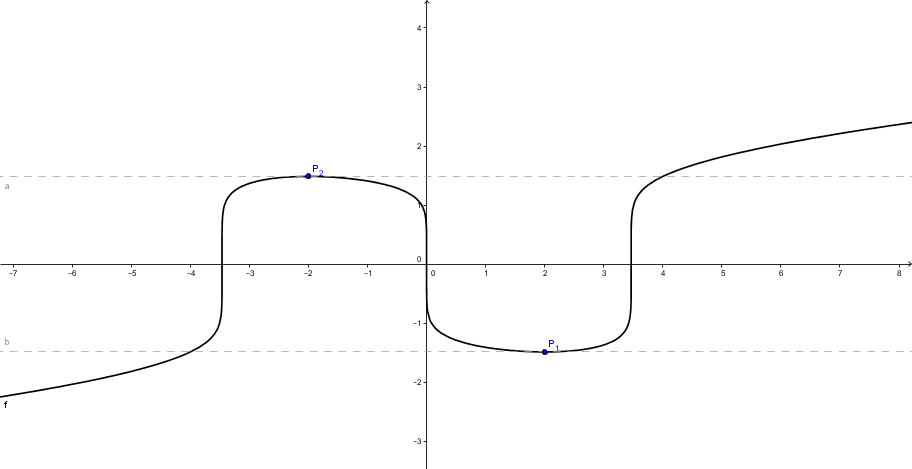
\includegraphics[scale=1.5]{img/5.png}
			$ P_1=(2, \sqrt[7]{-16} ) $\\
			$ P_2=(-2, \sqrt[7]{16} $\\
		\end{center}		
		
		\item Em que pontos a função $f$ é derivável?\\
		\\
		A função $f$ só não é derivável nos pontos onde o denominador é zero, ou seja:
		
		\begin{center}
			$ 7(x^3 - 12x)^{\frac{6}{7}} = 0 $\\
			$ x^3 - 12x = 0 $\\
			$ x = 0, x = \sqrt{12}, x = -\sqrt{12}$\\
		\end{center}
		
		Logo $f$ é derivável em $\mathbb{R} / x \not= 0, x \not= \sqrt{12}, x \not= -\sqrt{12}$\\
	\end{enumerate}
	\item (4,0 pontos) Considere a função $ f(x) = x^2 - x -2 $. Mostre que $f(x)$ possui pelo menos duas raízes reais distintas.\\
	\\
	Como $f$ é uma função polinomial é contínua.\\
	\\
	Basta tomar $f(-2) = 4$, $f(0) = -2$ e $f(3) = 4$, pelo teorema do valor intermediário podemos dizer que entre  $f(-2)$ e $f(0)$ há uma raiz, pois entre dois pontos de sinais opostos na imagem, sendo a função $f$ contínua deve haver uma raiz no intervalo. Da mesma forma afirmamos que há uma raiz entre $f(0)$ e $f(3)$. Logo $ f(x) = x^2 - x -2 $ possui duas raízes reais distintas, já que os intervalos $(-2,0)$ e $(0,3)$ não se interceptam.
	
	\begin{center}
		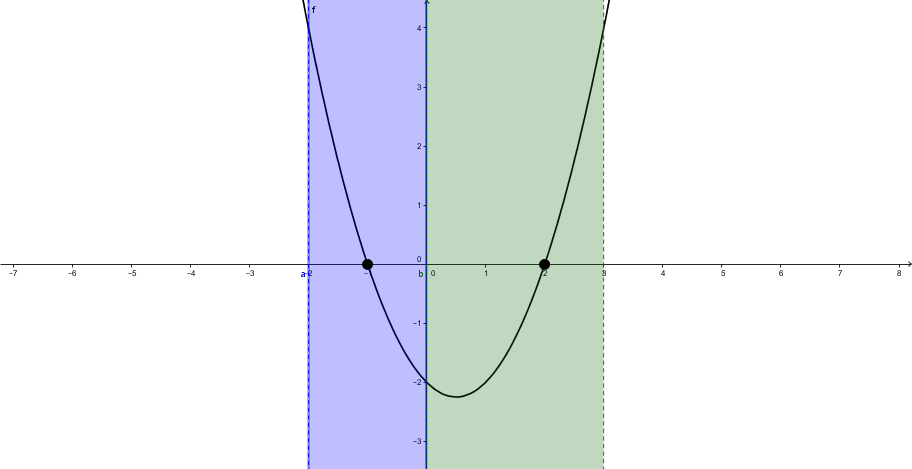
\includegraphics[scale=1.5]{img/6.png}
	\end{center}	
\end{enumerate}


\end{document}